\setchapterstyle{kao}
\setchapterpreamble[u]{\margintoc}

\chapter{PWM Generation}

The main task of the \gls{midi}-Interrupter is to create four PWM signals with frequencies within the audio range and variable duty cycles to change the volume of each tone. Those separate channels had then to be merged into a single channel, while preserving the original frequencies as much as possible without distorting them.

\section{Timers}

\subsection{Mode of Operation}

The 16 bit timers of the ATmega2560 have five modes of operation. Each one differs in complexity and flexibility. However, one thing they all have in common is the Output Compare Unit. It constantly compares the counter value to the value set in the \cinl{OCRnx} register. The unit can be configured to either generate an interrupt or set, clear, or toggle the corresponding \cinl{OCnx} pin when a compare match occurs.

\begin{enumerate}
    \item The \textbf{Normal Mode} counts from zero to 2\textsuperscript{16}-1, sets an overflow flag, and jumps back to zero. Because it can only count at a few fixed speeds and because using a compare match Unit in this mode is not recommended, it cannot produce the desired waveforms.
    \item The \textbf{CTC Mode}, also called \enquote{clear timer on compare match}, counts up until a compare match occurs and then resets to zero. Since the value to compare to can be set by the user, this allows for variable frequencies, however the duty cycle will always be 50\%.
    \item The \textbf{Fast PWM Mode} counts from zero to TOP, which can be set by the user, and then resets back to zero. By setting a compare match somewhere between zero and TOP, \cinl{OCRnx} can be set on compare match and cleared at TOP. This way, both a variable frequency and a variable duty cycle can be generated.\label{itm:fpm}
    \item The \textbf{Phase Correct PWM Mode} counts from zero to TOP and then back to zero. While upcounting, \cinl{OCRnx} will be set on compare match, and while downcounting, \cinl{OCRnx} will be cleared. Since one period in this mode is twice as long as in the previous modes, the timer acts like a 17 bit timer, which doubles its accuracy.\label{itm:pcm} % explain why we don't use this mode already
    \item The \textbf{Phase and Frequency Correct PWM Mode} is almost the same as mode \ref{itm:pcm}, except that \cinl{OCRnx} and TOP are updated on BOTTOM instead of on TOP.\label{itm:pfcm}
\end{enumerate}

Both mode \ref{itm:pcm} and \ref{itm:pfcm} can either use \cinl{ICRn} or \cinl{OCRnA} as TOP. \cinl{ICRn} is not double buffered, meaning that its value will be updated immediately when written. This could lead to issues, e.g., the timer is upcounting, and TOP is set to a lower value than the counter value. The timer will then miss TOP and count to 2\textsuperscript{16}-1, which has an impact on the generated PWM signal. A double buffered register like \cinl{OCRnA} can be used to mitigate this issue. In this case, TOP will not be updated until the timer reaches either TOP in mode \ref{itm:pcm} or BOTTOM in mode \ref{itm:pfcm}. The disadvantage of using \cinl{OCRnA} is that it is not possible anymore to use the Output Compare Unit A. However, this is not a problem since only one PWM signal per timer is needed.

To summarize, modes \ref{itm:fpm}, \ref{itm:pcm}, and \ref{itm:pfcm} would be able to generate the desired waveforms. However, modes \ref{itm:pcm} and \ref{itm:pfcm} are twice as accurate as mode \ref{itm:fpm}. Despite their names \enquote{Phase correct} and \enquote{Phase and Frequency correct}, the latter mode isn't more frequency correct than the former. They can be equally correct or incorrect depending on whether the TOP register is double-buffered. There is practically no difference between those two, except for the time the registers are updated. The datasheet, however, states that

\begin{displayquote}
\enquote{It is recommended to use the phase and frequency correct mode instead of the phase correct mode when changing the TOP value while the Timer/Counter is running.}
\end{displayquote}

Since this is the case for the \gls{midi}-Interrupter, the \textbf{Phase and Frequency Correct PWM Mode} was chosen. Its timing diagram can be seen in figure \ref{fig:timer_diagram}.

\begin{figure}[h!]
    \centering
    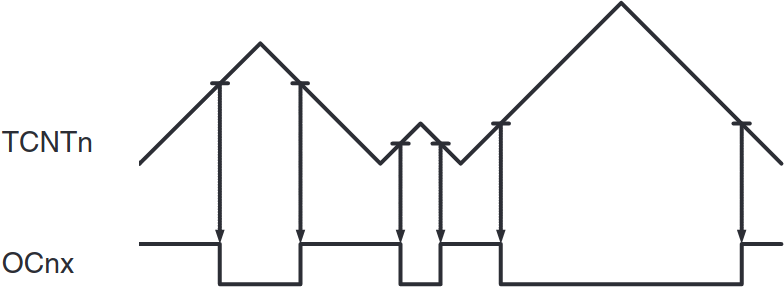
\includegraphics[width=0.9\textwidth]{felix/resources/timer_diagram.png}
    \caption{Timing diagram of the Phase and Frequency correct PWM mode}
    \label{fig:timer_diagram}
\end{figure}

\subsection{Prescaler}

The \gls{midi} protocol can encode frequencies from about 8 Hz to 13 kHz, which the timers should cover. To reach this range, a prescaler can be used, which sets the counting speed of the timers to a fraction of the clock speed. Table \ref{tab:prescaler} shows all possible prescalers and their resulting frequency ranges.

Note that the maximum frequency is not actually the highest frequency possible for each prescaler. This is because the lower the number of steps, until TOP is reached, the lower the number of possible duty cycles. To ensure that the duty cycle resolution is at least 2\% for every frequency, the minimum number of steps for each period was set to 100, which effectively divides the theoretically highest possible frequency by twenty-five.

\begin{table}[h!]
    \centering
    \begin{tabular}{@{}rrrrr@{}}
        \textbf{Prescaler} & \textbf{Counting Frequency} & \textbf{Resolution} & \textbf{f\textsubscript{min}} & \textbf{f\textsubscript{max}} \\\midrule
        1 & 16 MHz & 62.5 ns & 122 Hz & 160 kHz \\
        8 & 2 MHz & 500 ns & 15.3 Hz & 20 kHz \\
        64 & 250 kHz & 4 \textmu s & 1.91 Hz & 2.5 kHz \\
        256 & 62.5 kHz & 16 \textmu s & 0.48 Hz & 625 Hz \\
        1024 & 15.625 kHz & 64 \textmu s & 0.12 Hz & 156 Hz \\
    \end{tabular}
    \caption{Prescalers}
    \label{tab:prescaler}
\end{table}

The only prescaler within the desired frequency range was the \textbf{prescaler 8}.

\subsection{Output Compare Pins}

Each timer has three output compare units - A, B, and C - each with their own pin, OCnA, OCnB, and OCnC, respectively. Unit B was chosen for all timers, whose pins can be seen in table \ref{tab:compare-pins}.

\begin{margintable}[-3cm]
\centering
\caption{Output compare pins\label{tab:compare-pins}}
\begin{tabular}{cc}
    \textbf{MCU pin} & \textbf{Arduino pin}\\\midrule
    OC1B & 12\\
    OC3B & 2\\
    OC4B & 7\\
    OC5B & 39
\end{tabular}
\end{margintable}

\section{Using the Timers}

To use the timers in a convenient way, a timer handler has been implemented, as shown in listing \ref{lst:pwmtimer}.

\begin{lstlisting}[caption=PWMTimer class, label=lst:pwmtimer]
// Constructor
PWMTimer::PWMTimer(uint16_t _ocnb_port_addr,
				   uint16_t _ocnb_pin_addr,
				   uint16_t _top_addr,
				   uint16_t _com_addr,
				   uint16_t _TCCRnA_addr,
				   uint16_t _TCCRnB_addr, 
				   uint16_t _TCNTn_addr) {
    // Save register addresses for later
    top_addr = _top_addr;
    com_addr = _com_addr;
    TCCRnB_addr = _TCCRnB_addr;
    TCNTn_addr = _TCNTn_addr;
    // Set OCnx as output
    _SFR_MEM8(_ocnb_port_addr) |= (1 << _ocnb_pin_addr);
    // Set Phase and Frequency correct PWM Mode with OCRnA as TOP
    _SFR_MEM16(_TCCRnA_addr) |= (1 << WGMn0);
    _SFR_MEM16(_TCCRnB_addr) |= (1 << WGMn3);
    // Clear OCnB on Compare Match when upcounting, set when downcounting
    _SFR_MEM16(_TCCRnA_addr) |= (1 << COMnB1);
}

void PWMTimer::start(uint16_t freq, uint8_t duty_cycle) {
    isFree = false;
    uint16_t top = 1000000 / freq;
    _SFR_MEM16(top_addr) = top;
    _SFR_MEM16(com_addr) = top * duty_cycle / 100;
    // Set prescaler to 8 to start timer
    _SFR_MEM8(TCCRnB_addr) |= (1 << CSn1);
}

void PWMTimer::stop() {
    // Wait until OCnB is low, before turning off the timer
    while(_SFR_MEM16(TCNTn_addr) < (top * duty_cycle / 100));
    // Set prescaler to 0 to stop the timer
    _SFR_MEM8(TCCRnB_addr) &= ~(1 << CSn1);
    isFree = true;
}
\end{lstlisting}

Each timer is its own instance of the \cinl{PWMTimer} class. To still access all registers, the register addresses were passed to the constructor. Instead of writing, e.g., \cinl{DDRB}, which is just defined as \cinl{_SFR_MEM8(0x24)}, the macros \cinl{_SFR_MEM8}, and \cinl{_SFR_MEM16} are used directly with the register address.

To ensure that \cinl{OCnx} is low when the timer turns off, which will be important in section \ref{sec:signal-combination}, the turn-off will be delayed until the counter value is bigger than \cinl{OCRnx}, which means that \cinl{OCnx} has been cleared.

Starting and Stoping every timer manually is still a bit tedious, so an additional layer of abstraction was created. This layer was implemented as a namespace, which can be seen as a singleton because it does not have to be instantiated.

\begin{lstlisting}[caption=PWM namespace, label=lst:pwm-namespace]
namespace PWM {
	namespace {
		PWMTimer timers[4];
	}
	void init();
	void start(uint16_t freq, uint8_t dc = 20);
	void stop(uint16_t freq);
}

void PWM::init() {
    timers[0] = PWMTimer(/* List of register addresses */);
	timers[1] = PWMTimer(/* List of register addresses */);
	timers[2] = PWMTimer(/* List of register addresses */);
	timers[3] = PWMTimer(/* List of register addresses */);
}

void PWM::start(uint16_t freq, uint8_t dc) {
    // Start the first free timer
    for(PWMTimer & timer : timers) {
        if(timer.isFree) {
            timer.start(freq, dc);
            break;
        }
    }
}

void PWM::stop(uint16_t freq) {
    // Stop the timer playing this frequency
    for(PWMTimer & timer : timers) {
        if(timer.freq == freq) {
            timer.stop();
            break;
        }
    }
}
\end{lstlisting}

Unfortunately, most C\texttt{++} standard libraries are not available for the AVR platform, so instead of storing the timers in a \cinl{std::vector<PWMTimer>}, they had to be stored in a fixed-size C array.

This namespace allows easy control over the timers as shown in listing \ref{lst:pwm-namespace-usage}.

\begin{lstlisting}[caption=PWM namespace usage, label=lst:pwm-namespace-usage]
PWM::start(500); // Starts Timer 1
PWM::start(600); // Starts Timer 2
PWM::stop(500);  // Stops  Timer 1
PWM::start(700); // Starts Timer 1
PWM::start(800); // Starts Timer 3
\end{lstlisting}

\section{Signal Combination}
\label{sec:signal-combination}

% mention input duty cycle and using an AND gate

At the moment, the MIDI-Interrupter can create four PWM signals on four separate pins. However, the tesla coil needs to be fed a single PWM signal. Unlike regular music consisting of a series of sine waves, logic signals cannot be added as easily. One approach would be to convert every PWM signal into a sine wave where the duty cycle corresponds to the amplitude. Those sine waves are then added together, and for each point, if the result is above a specific threshold, the output signal is high, else it is low.

However, this would be very computation-intensive task and would likely require an additional \gls{mcu}. Instead, a simpler yet effective method was chosen - using logic gates. Just like how a specific PWM frequency modulated onto a higher PWM carrier frequency creates a sound that contains both frequencies\sidenote{This was explained in detail in section \ref{sec:musical-tesla-coils}}, all four PWM channels can be merged using an OR gate. If only one channel is playing, then it is just passing through without any change. If two or more channels are playing, they get overlapped and therefore are all contained in the output signal. 

\begin{figure}[h!]
    \centering
    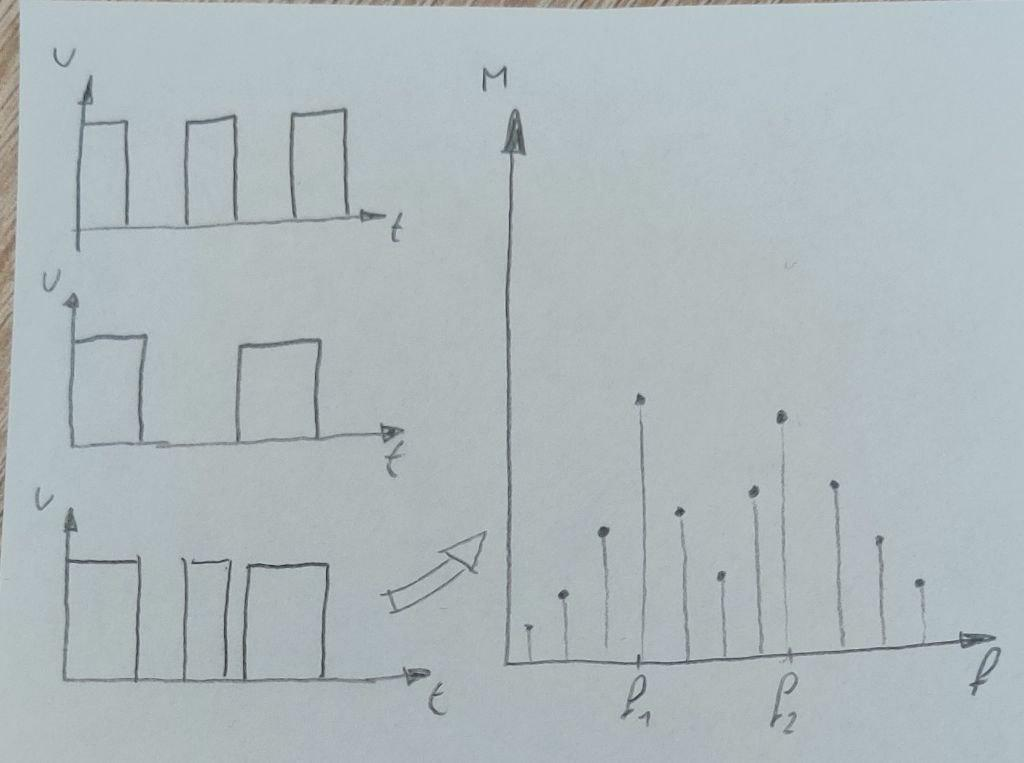
\includegraphics[width=0.7\textwidth]{felix/resources/signalCombinationFourier.jpg}
    \caption{Frequency Components of the Output Signal}
    \label{fig:signal-combination-fourier}
\end{figure}

This merging can also be thought of as adding the PWM signals together like analog signals and then just cutting away everything above the previous logic 1 level. However, this also leads to a problem because information is being destroyed every time something is cut away from the waveform. This result is either added unwanted frequency components, removed wanted frequency components, or both. In the worst case, if one frequency is an integer multiple of the other and they are in phase, they overlap so that the lower frequency will get removed entirely. In the same way, if they are exactly out of phase, it will seem like another, higher frequency had been added.

% add moer fourier stuff

Despite the seemingly bad quality of the output signal, all input frequencies are clearly audible when played on a buzzer, and the distortions hardly could be noticed.